\begin{comment}
\end{comment}

\chapter{Comptage variationnel quantique}

%-----------------------------------------------------------------------------%

\subsection*{Plan}

\begin{enumerate}
    \item Expliquer que cette section ne concerne que GM-QAOA
\end{enumerate}

%-----------------------------------------------------------------------------%

\section{Algorithme VQCount}

\subsection*{Plan}

\begin{enumerate}
    \item Vulgariser l'algorithme de manière général
    \item Expliquer rigoureusement l'algorithme
    \item Faire le lien entre la notation utilisée dans les algorithmes de comptage classique
    \item Faire la comparaison avec les travaux précédents
    \item Rajouter l'algorithme complet en pseudo-code
\end{enumerate}

\subsection*{Références}

% \begin{figure}[t]
%     \centering
%     \begin{quantikz}[font=\sffamily]
%       \ket{0} & \gate[style={fill=mysilver!80}][0.80cm]{H} & \gate[wires=4, nwires=3, style={fill=myblue}][1.30cm]{U_P (\alpha_{1})} & \gate[wires=4, nwires=3, style={fill=myred}][1.30cm]{U_D (\beta_{1})} & \ \ldots\ \qw & \gate[wires=4, nwires=3, style={fill=myblue}][1.30cm]{U_P (\alpha_{p})} & \gate[wires=4, nwires=3, style={fill=myred}][1.30cm]{U_D (\beta_{p})} & \qw \\
%       \ket{0} & \gate[style={fill=mysilver!80}][0.80cm]{H} & & & \ \ldots\ \qw & & & \qw \\
%       \vdots & & & & & & & \\
%       \ket{0} & \gate[style={fill=mysilver!80}][0.80cm]{H} & & & \ \ldots\ \qw & & & \qw
%     \end{quantikz}
%     \caption{}
% \end{figure}

% \begin{figure}[t]
%     \centering
%     \begin{quantikz}
%       \ket{0} & \gate[style={fill=myyellow!80}][0.80cm]{X^{c}} & \gate[wires=4, nwires=3, style={fill=myblue}][1.30cm]{U_P (\alpha_{1})} & \qw & \ \ldots\ \qw & \gate[wires=4, nwires=3, style={fill=myblue}][1.30cm]{U_P (\alpha_{p}) } & \qw & \qw \\
%       \ket{0} & \gate[style={fill=mysilver!80}][0.80cm]{H} & & \gate[wires=3, nwires=2, style={fill=myred}][1.30cm]{U_D (\beta_{1})} & \ \ldots\ \qw & & \gate[wires=3, nwires=2, style={fill=myred}][1.30cm]{U_D (\beta_{p})} & \qw \\
%       \vdots & & & & & & & \\
%       \ket{0} & \gate[style={fill=mysilver!80}][0.80cm]{H} & & & \ \ldots\ \qw & & & \qw
%     \end{quantikz}
%     \caption{}
% \end{figure}

% \begin{figure}[h]
%     \centering
%     \begin{quantikz}
%         \ket{x_1} & \ctrl{3} & \qw      & \qw      & \qw      & \qw      & \qw      & \qw      & \qw & \qw \\
%         \ket{x_2} & \qw      & \ctrl{2} & \ctrl{3} & \qw      & \qw      & \qw      & \qw      & \qw & \qw \\
%         \ket{x_3} & \qw      & \qw      & \qw      & \ctrl{2} & \qw      & \qw      & \qw      & \qw & \qw \\
%         \ket{0}   & \targ{}  & \targ{}  & \qw      & \qw      & \targ{}  & \ctrl{2}      & \qw      & \qw & \qw \\
%         \ket{0}   & \qw      & \qw      & \targ{}  & \targ{}  & \targ{}  & \ctrl{1}       & \qw     & \qw & \qw \\
%         \ket{0}   & \qw      & \qw      & \qw      & \qw      & \qw      & \targ{}       & \ctrl{7} & \qw & \qw \\ [0.5cm]
%         \ket{x_1} & \ctrl{3} & \qw      & \qw      & \qw      & \qw      & \qw      & \qw      & \qw & \qw \\
%         \ket{x_2} & \qw      & \ctrl{2} & \ctrl{3} & \qw      & \qw      & \qw      & \qw      & \qw & \qw \\
%         \ket{x_3} & \qw      & \qw      & \qw      & \ctrl{2} & \qw      & \qw      & \qw      & \qw & \qw \\
%         \ket{0}   & \targ{}  & \targ{}  & \qw      & \qw      & \targ{}  & \ctrl{2}      & \qw      & \qw & \qw \\
%         \ket{0}   & \qw      & \qw      & \targ{}  & \targ{}  & \targ{}  & \ctrl{1}       & \qw     & \qw & \qw \\
%         \ket{0}   & \qw      & \qw      & \qw      & \qw      & \qw      & \targ{}       & \ctrl{1}  & \qw & \qw \\ [0.5cm]
%         \ket{0}   & \qw      & \qw      & \qw      & \qw      & \qw      & \qw      & \gate{Z^{- \gamma \varepsilon/\pi}}  & \meter{} & \qw \\
%         \end{quantikz}
%     \caption{}
%     \label{fig:...}
% \end{figure}

% \begin{figure}[h]
%     \centering
%     \begin{quantikz}
%         \ket{x_1} & \ctrl{3} & \qw      & \qw      & \qw      & \qw      & \qw      & \qw      & \qw      & \qw      & \qw      & \qw      & \qw     & \ctrl{3} & \qw \\
%         \ket{x_2} & \qw      & \ctrl{2} & \ctrl{3} & \qw      & \qw      & \qw      & \qw      & \qw      & \qw      & \qw      & \ctrl{3} & \ctrl{2}     & \qw      & \qw \\
%         \ket{x_3} & \qw      & \qw      & \qw      & \ctrl{2} & \qw      & \qw      & \qw      & \qw      & \qw      & \ctrl{2} & \qw      & \qw     & \qw      & \qw \\
%         \ket{0}   & \targ{}  & \targ{}  & \qw      & \qw      & \targ{}  & \ctrl{2}      & \qw      & \ctrl{2} & \targ{}  & \qw      & \qw      & \targ{}      & \targ{}  & \qw \\
%         \ket{0}   & \qw      & \qw      & \targ{}  & \targ{}  & \targ{}  & \ctrl{1}      & \qw     & \ctrl{1}  & \targ{}  & \targ{}  & \targ{}  & \qw     & \qw     & \qw \\
%         \ket{0}   & \qw      & \qw      & \qw      & \qw      & \qw      & \targ{}       & \ctrl{7} & \targ{}  & \qw      & \qw      & \qw      & \qw     & \qw      & \qw \\ [0.5cm]
%         \ket{x_4} & \ctrl{3} & \qw      & \qw      & \qw      & \qw      & \qw      & \qw      & \qw      & \qw      & \qw      & \qw      & \qw     & \ctrl{3} & \qw \\
%         \ket{x_5} & \qw      & \ctrl{2} & \ctrl{3} & \qw      & \qw      & \qw      & \qw      & \qw      & \qw      & \qw      & \ctrl{3} & \ctrl{2}     & \qw      & \qw \\
%         \ket{x_6} & \qw      & \qw      & \qw      & \ctrl{2} & \qw      & \qw      & \qw      & \qw      & \qw      & \ctrl{2} & \qw      & \qw     & \qw      & \qw \\
%         \ket{0}   & \targ{}  & \targ{}  & \qw      & \qw      & \targ{}  & \ctrl{2}      & \qw      & \ctrl{2} & \targ{}  & \qw      & \qw      & \targ{}      & \targ{}  & \qw \\
%         \ket{0}   & \qw      & \qw      & \targ{}  & \targ{}  & \targ{}  & \ctrl{1}      & \qw     & \ctrl{1}  & \targ{}  & \targ{}  & \targ{}  & \qw     & \qw     & \qw \\
%         \ket{0}   & \qw      & \qw      & \qw      & \qw      & \qw      & \targ{}       & \ctrl{1} & \targ{}  & \qw      & \qw      & \qw      & \qw     & \qw      & \qw \\ [0.5cm]
%         \ket{0}   & \qw      & \qw      & \qw      & \qw      & \qw      & \qw      & \gate{Z^{- \gamma \varepsilon/\pi}}  & \qw & \qw & \qw & \qw & \qw & \meter{} & \qw \\
%         \end{quantikz}
%     \caption{}
%     \label{fig:..}
% \end{figure}

\begin{figure*}[t]
    \centering
    \begin{subfigure}[h]{0.45\textwidth}
    \centering
    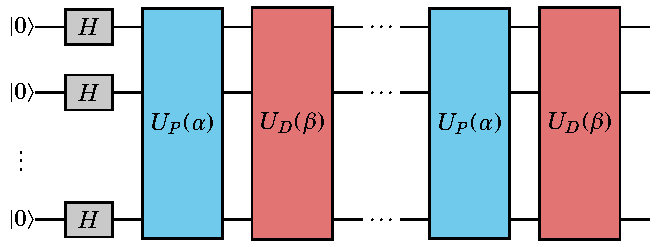
\includegraphics[width=1\textwidth]{figures/qaoa-self-reducibility-1.pdf}
    \caption{}
    \label{fig:quantum-circuit-a}
    \end{subfigure}
    \begin{subfigure}[h]{0.45\textwidth}
    \centering
    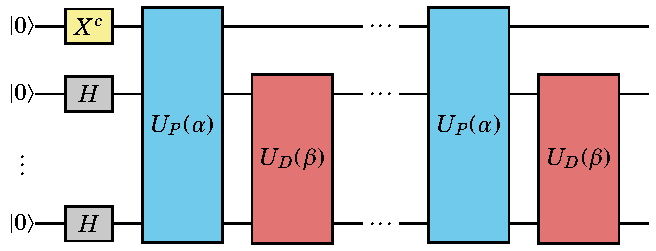
\includegraphics[width=1\textwidth]{figures/qaoa-self-reducibility-2.pdf}
    \caption{}
    \label{fig:quantum-circuit-b}
    \end{subfigure}
\caption{}
\label{fig:quantum-circuit}
\end{figure*}

\begin{figure*}[h]
    \centering
    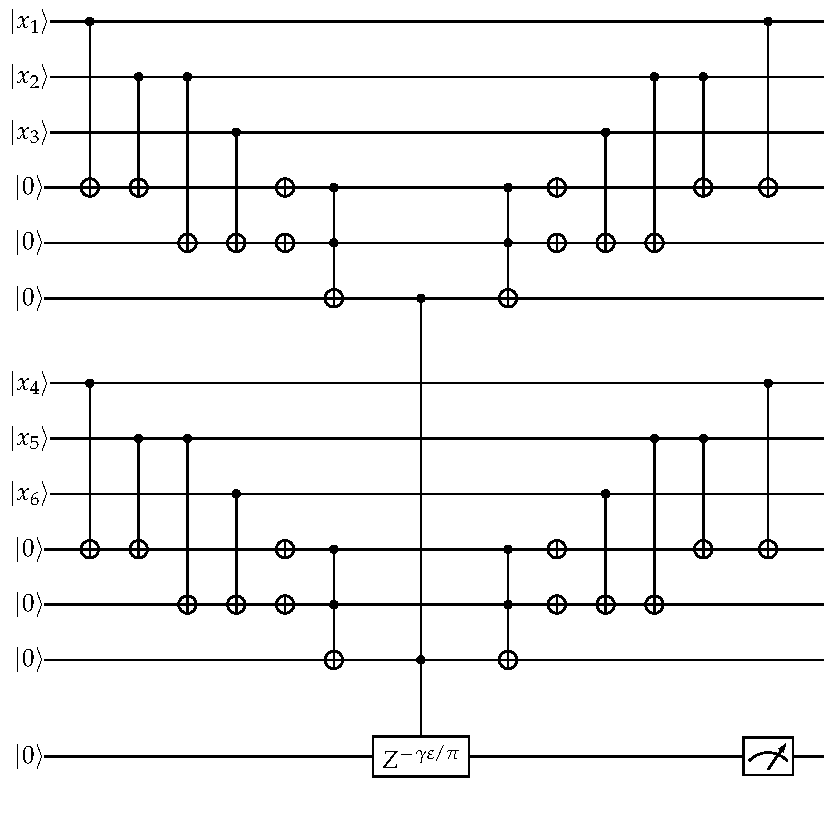
\includegraphics[width=0.6\textwidth]{figures/two-level-map.pdf}
    \caption{}
    \label{fig:two-level-map}
\end{figure*}

%-----------------------------------------------------------------------------%

\section{Auto-réductibilité des algorithmes variationnels quantiques}

\subsection*{Plan}

\begin{enumerate}
    \item Faire la preuve de l'auto-réductibilité des algorithmes variationnels quantiques
\end{enumerate}

\subsection*{Références}

%-----------------------------------------------------------------------------%

\section{Module VQCount}

\subsection*{Plan}

\begin{enumerate}
    \item Expliquer les librairies python dévelopées
    \item Décrire \textit{qaoa-quimb}
    \item Décrire \textit{VQCount}
\end{enumerate}

\subsection*{Références}